\begin{enumerate}[label=\thesubsection.\arabic*, ref=\thesubsection.\theenumi]
    
    \item If $x = \alpha$ is a root of $ax^2 + bx + c = 0$, substituting $x = \alpha$ satisfies:
\begin{align}
    a\alpha^2 + b\alpha + c = 0 \label{eq:EE26BTECH11225-root}
\end{align}

    \item If $\alpha$ and $\beta$ are zeroes of $p(x)$, then $(x - \alpha)(x - \beta)$ is a factor of $p(x)$.
\begin{align}
    p(x) = (x - \alpha)(x - \beta)\,q(x) \label{eq:EE26BTECH11225-factor}
\end{align}

    \item Roots of a quadratic equation $ax^2 + bx + c = 0$ ($a \neq 0$) and nature of roots:
\begin{align}
    x &= \frac{-b \pm \sqrt{b^2 - 4ac}}{2a} \label{eq:EE26BTECH11225-quadratic} \\
    D > 0 &\implies \text{two distinct real roots} \nonumber \\
    D = 0 &\implies \text{two equal real roots} \nonumber \\
    D < 0 &\implies \text{no real roots} \nonumber
\end{align}

    \item The $n^{\text{th}}$ term $a_n$ of an Arithmetic Progression (A.P.):
\begin{align}
    a_n = a + (n - 1)d \label{eq:EE26BTECH11225-ap-nth}
\end{align}

    \item Sum of the first $n$ terms $S_n$ of an A.P.:
\begin{align}
    S_n = \frac{n}{2}[2a + (n - 1)d] = \frac{n}{2}(a + l) \label{eq:EE26BTECH11225-ap-sum}
\end{align}
where $l = a_n$ is the last term.

    \item Four consecutive terms in an A.P. with common difference $2d$:
\begin{align}
    (a - 3d), \quad (a - d), \quad (a + d), \quad (a + 3d) \label{eq:EE26BTECH11225-ap-four}
\end{align}

    \item Distance between points $P(x_1, y_1)$ and $Q(x_2, y_2)$:
\begin{align}
    d = \sqrt{(x_2 - x_1)^2 + (y_2 - y_1)^2} \label{eq:EE26BTECH11225-distance}
\end{align}

    \item Section formula for internal division in ratio $k : 1$:
\begin{align}
    x = \frac{k x_2 + x_1}{k + 1}, \quad y = \frac{k y_2 + y_1}{k + 1} \label{eq:EE26BTECH11225-section}
\end{align}

    \item The area of a triangle with vertices $(x_1, y_1)$, $(x_2, y_2)$, and $(x_3, y_3)$ is:
\begin{align}
    \text{Area}(\Delta) = \frac{1}{2} |x_1(y_2 - y_3) + x_2(y_3 - y_1) + x_3(y_1 - y_2)| \label{eq:EE26BTECH11225-area-triangle}
\end{align}
The area of quadrilateral $ABCD$ is computed as:
\begin{align}
    \text{Area}(ABCD) = \text{Area}(\Delta ABC) + \text{Area}(\Delta ADC) \label{eq:EE26BTECH11225-area-quad}
\end{align}

    \item Area Ratio Theorem for similar triangles ($\Delta ABC \sim \Delta PQR$):
\begin{align}
    \frac{\text{ar}(\Delta ABC)}{\text{ar}(\Delta PQR)} = \left(\frac{AB}{PQ}\right)^2 \label{eq:EE26BTECH11225-area-ratio}
\end{align}
\textbf{Proof:} \\
Draw altitudes $AM \perp BC$ and $PN \perp QR$.
\begin{align}
    \frac{\text{ar}(\Delta ABC)}{\text{ar}(\Delta PQR)} = \frac{\frac{1}{2} \cdot BC \cdot AM}{\frac{1}{2} \cdot QR \cdot PN} = \left(\frac{BC}{QR}\right) \left(\frac{AM}{PN}\right) \nonumber
\end{align}
Since $\Delta ABM \sim \Delta PQN$, we have $\frac{AM}{PN} = \frac{AB}{PQ} = \frac{BC}{QR}$. Substituting yields:
\begin{align}
    \frac{\text{ar}(\Delta ABC)}{\text{ar}(\Delta PQR)} = \left(\frac{AB}{PQ}\right)^2 \nonumber
\end{align}

    \item Tangent properties of a circle:
    \begin{center}
    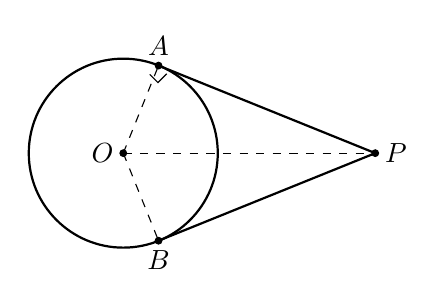
\begin{tikzpicture}[scale=0.8]
        \draw[thick] (0,0) circle (1.5cm);
        \coordinate (O) at (0,0);
        \coordinate (P) at (4,0);
        \coordinate (A) at (0.56, 1.39);
        \coordinate (B) at (0.56, -1.39);
        
        \draw[dashed] (O) -- (A);
        \draw[dashed] (O) -- (B);
        \draw[dashed] (O) -- (P);
        \draw[thick] (P) -- (A);
        \draw[thick] (P) -- (B);
        
        \filldraw (O) circle (1.5pt) node[left] {$O$};
        \filldraw (P) circle (1.5pt) node[right] {$P$};
        \filldraw (A) circle (1.5pt) node[above] {$A$};
        \filldraw (B) circle (1.5pt) node[below] {$B$};
        
        % Right angle symbol at A
        \draw (0.42,1.25) -- (0.55,1.12) -- (0.69,1.26);
    \end{tikzpicture}

    \end{center}
    Radius is perpendicular to tangent at point of contact:
\begin{align}
    \angle OAP = 90^\circ \label{eq:EE26BTECH11225-tangent-perp}
\end{align}
    Tangents drawn to a circle from an external point $P$ will be equal in length:
\begin{align}
    PA = PB \label{eq:EE26BTECH11225-tangent-equal}
\end{align}

    \item Pythagoras Theorem in a right-angled triangle:
\begin{align}
    \text{Hypotenuse}^2 = \text{Base}^2 + \text{Height}^2 \label{eq:EE26BTECH11225-pythagoras}
\end{align}

    \item Fundamental trigonometric identities and standard ratios:
\begin{align}
    \sin^2 A + \cos^2 A &= 1 \label{eq:EE26BTECH11225-trig-1} \\
    \sec^2 A - \tan^2 A &= 1 \label{eq:EE26BTECH11225-trig-2} \\
    \csc^2 A - \cot^2 A &= 1 \label{eq:EE26BTECH11225-trig-3}
\end{align}
\begin{align}
    \tan\theta = \frac{\text{Opposite}}{\text{Adjacent}}, \quad \sin\theta = \frac{\text{Opposite}}{\text{Hypotenuse}}, \quad \cos\theta = \frac{\text{Adjacent}}{\text{Hypotenuse}} \label{eq:EE26BTECH11225-trig-ratios}
\end{align}

    \item Complementary angle identities:
\begin{align}
    \cos(90^\circ - \theta) = \sin\theta, \quad \tan(90^\circ - \theta) = \cot\theta \label{eq:EE26BTECH11225-complementary}
\end{align}

    \item Area of a circular sector with central angle $\theta$:
\begin{align}
    \text{Area} = \frac{\theta}{360^\circ} \times \pi r^2 \label{eq:EE26BTECH11225-sector}
\end{align}
Four $90^\circ$ corner quadrants combine to form $1$ full circle of area $\pi r^2$.

    \item Surface areas of a cylinder and hemisphere:
\begin{align}
    \text{CSA of cylinder} &= 2\pi rh \label{eq:EE26BTECH11225-csa-cyl} \\
    \text{CSA of hemisphere} &= 2\pi r^2 \label{eq:EE26BTECH11225-csa-hemi}
\end{align}

    \item Volume, slant height, and curved surface area of a cone:
\begin{align}
    V &= \frac{1}{3}\pi r^2 h \label{eq:EE26BTECH11225-cone-vol} \\
    l &= \sqrt{r^2 + h^2}, \quad \text{CSA} = \pi r l \label{eq:EE26BTECH11225-cone-csa}
\end{align}

    \item Slant height and surface area of an open frustum:
\begin{align}
    l &= \sqrt{h^2 + (R - r)^2} \label{eq:EE26BTECH11225-frustum-l} \\
    \text{Area} &= \pi(R + r)l + \pi r^2 \label{eq:EE26BTECH11225-frustum-area}
\end{align}

    \item Classical probability and complementary event rule:
\begin{align}
    P(E) = \frac{n(E)}{n(S)} \label{eq:EE26BTECH11225-prob} \\
    \quad P(E') = 1 - P(E) \label{eq:EE26BTECH11225-prob-comp}
\end{align}

    \item Direct method for Mean and grouped Median formula:
\begin{align}
    \bar{x} &= \frac{\sum f_i x_i}{\sum f_i} \label{eq:EE26BTECH11225-mean} \\
    \text{Median} &= l + \left(\frac{\frac{N}{2} - cf}{f}\right) \times h \label{eq:EE26BTECH11225-median}
\end{align}
\end{enumerate}
